
CMEs

Another type of structure frequently found to be embedded in the slow and fast solar-wind streams are transient CMEs which have durations of a few days. CMEs make up about \SI{5}{\percent} of the solar wind's flow share during solar cycle minima, but can represent up to about \SI{50}{\percent} during solar cycle maxima \citep{Richardson2012}.\\

CMEs are eruptions of coronal magnetized plasma, which expand within hours to blobs with sizes of a few solar radii. They continuously expand further while moving farther away from the Sun into the heliosphere.\\

Long before the origins of magnetospheric disturbances were actually attributed to CMEs, the solar influence was identified as their source by \citet{Carrington1859}. Indeed, CMEs are the major drivers for strong geomagnetic disturbances, because they carry the most extreme conditions found in the solar wind. Thus, they are of major importance to space weather -- their impacts on the terrestrial magnetosphere are covered in the following \autoref{sec:space_weather}.\\

CMEs were detected in white-light observations made by the first space-based coronagraphs on board the OSO~7 satellite \citep{Tousey1973} and the Skylab space station \citep{MacQueen1974}. These observations show the steady outflow of solar wind, broken by intermittend ejections of coronal plasma. Subsequently, the kinematic properties of CMEs were identified from the white-light images \citep{MacQueen1980}. Now, coronagraphs observe the corona and hence CMEs continuously from the first Lagrange point in front of Earth with the SOHO spacecraft and from different equatorial perspectives with the STEREO~A and~B spacecraft. The image of the corona from 23~September 2012, made by the SECCHI/COR2 coronagraph onboard STEREO~A, shows a CME to the top right, see \autoref{fig:CME_COR2_0120923_182400_dbc2A}.\\
\begin{figure}[htb]
	\fcapside[\FBwidth]{
		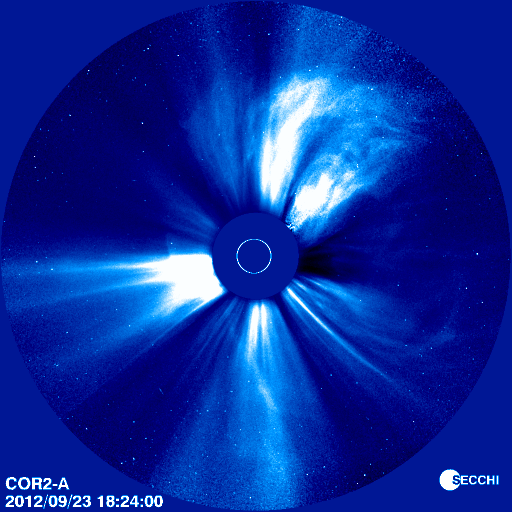
\includegraphics[width=0.6\textwidth]{figures_of_others/images/CME_COR2_0120923_182400_dbc2A.png}
	}{
		\caption{Image of the corona out to \SI{15}{\Rs} from 23~September 2012 made by the SECCHI/COR2 coronagraph onboard the STEREO~A spacecraft. The solar disk is covered by the occulter disk and its position is indicated by the white circle. The bright blob to the top right is the CME; the smooth elongated lines are solar wind streamers. Credit: NASA/STEREO... find optimal event... with shock and flux rope?}
		\label{fig:CME_COR2_0120923_182400_dbc2A}
	}
\end{figure}

It was early determined that solar ejecta should drive shock waves ahead \citep{Gold1962}. In fact, shocks with trailing low proton temperatures caused by fast CMEs were then found in in-situ measurements \citep{Gosling1973,Gosling1974}. Disturbances in front of fast CMEs can be identified as shocks in the white-light images of the newer SOHO coronagraph as well \citep{Sheeley2000}.\\




shocks
their white-light and in-situ structure
in-situ figure

flux-ropes/MCs
definition
orientation
BSS


associated events
flares
SEPs

surface formation
acceleration
interaction



extreme events

CME forecast
- frequency
- CME models

open questions
- formation
- acceleration


figures
- coronagraph perspectives + maybe annotated
- in-situ
- flux rope

